\documentclass[xcolor={usenames,dvipsnames},11pt]{beamer}

\defbeamertemplate{description item}{align left}{\insertdescriptionitem\hfill}

% \usetheme[sectionpage=none,subsectionpage=simple,progressbar=none,block=fill]{metropolis}
\usetheme[sectionpage=none,subsectionpage=simple,progressbar=frametitle,block=fill]{metropolis}
% \setsansfont[BoldFont={Fira Sans SemiBold}]{Fira Sans Book}
\usepackage{tikz}
\usetikzlibrary{patterns}
\usetikzlibrary{shapes.misc, positioning}
\usepackage{eso-pic}
\usepackage{booktabs}
\usepackage[scale=2]{ccicons}
\usepackage{pgfplots}
\usepackage{amsmath}
\usepackage{wasysym}
\usepackage{mathtools}
\usepackage{pgf}
\usepackage{pifont}
\usepackage{algpseudocode}
\usepackage{listings}
% \setsansfont{Ubuntu}
% \setmonofont{Ubuntu Mono}

\DeclarePairedDelimiter{\ceil}{\lceil}{\rceil}
\usepgfplotslibrary{dateplot}
\hypersetup{colorlinks,linkcolor=Cerulean,urlcolor=Cyan}

\usepackage{xspace}
\newcommand{\themename}{\textbf{\textsc{metropolis}}\xspace}
\usefonttheme[onlymath]{serif}
\setbeamertemplate{caption}{\raggedright\insertcaption\par}

\usepackage{tikz,pgfplots,filecontents}
\pgfplotsset{compat=1.7} 
\usepgfplotslibrary{colorbrewer}

\title{ \LARGE Design of Real-time Optical Coherence Tomography}
% \title{\LARGE Reccomendation for Space Data System Standards}
% \title{\Large Metropolis}
\subtitle{Master Thesis in Telecommunication Engineering\\ Department of Information Engineering}
\author[G. Marcon]{Master candidate: \textbf{Gianluca Marcon} \\ Supervisor: \textbf{Prof. Luca Palmieri}}
\date{\vspace{0.5cm}\centering April 18, 2018\vspace*{-0.5cm}}
%\institute{University of Padova}
% \institute{Department of Information Engineering, University of Padova}

% logo on every page
%\newcommand{\nologo}{\setbeamertemplate{logo}{}}

%\newcommand\AtPagemyUpperLeft[1]{\AtPageLowerLeft{%
%\put(\LenToUnit{0.94\paperwidth},\LenToUnit{0.03\paperheight}){#1}}}
%\AddToShipoutPictureFG{
%  \AtPagemyUpperLeft{{\includegraphics[height=2cm,keepaspectratio]{./logos/DEI.png}}}
%}%

\logo{\vspace*{-1.4cm}
\includegraphics[height=2cm,keepaspectratio]{./logos/DEI-moodle.png}}


% full logo on title page
\titlegraphic{
\includegraphics[height=2cm]{./logos/unipd}\hfill\raisebox{0.5cm}{
\includegraphics[width=5cm]{./logos/peg}}\hfill
\includegraphics[height=2cm]{./logos/DEI_full}}
\setbeamertemplate{subsection page}[simple]

\begin{document}

\maketitle

%======================================================================================
\section{Introduction}
\begin{frame}{Standard specifications}
    The standard specifies different input packet lengths $k$
    \begin{itemize}
        \item $1784$
        \item $3568$
        \item $7136$
        \item $8920$
    \end{itemize}

    ...and different code rates $R$
    \begin{itemize}
        \item $1/2$
        \item $1/3$
        \item $1/4$
        \item $1/6$
    \end{itemize}    
\end{frame}
%======================================================================================
\begin{frame}{Encoder structure}
    \begin{center}
        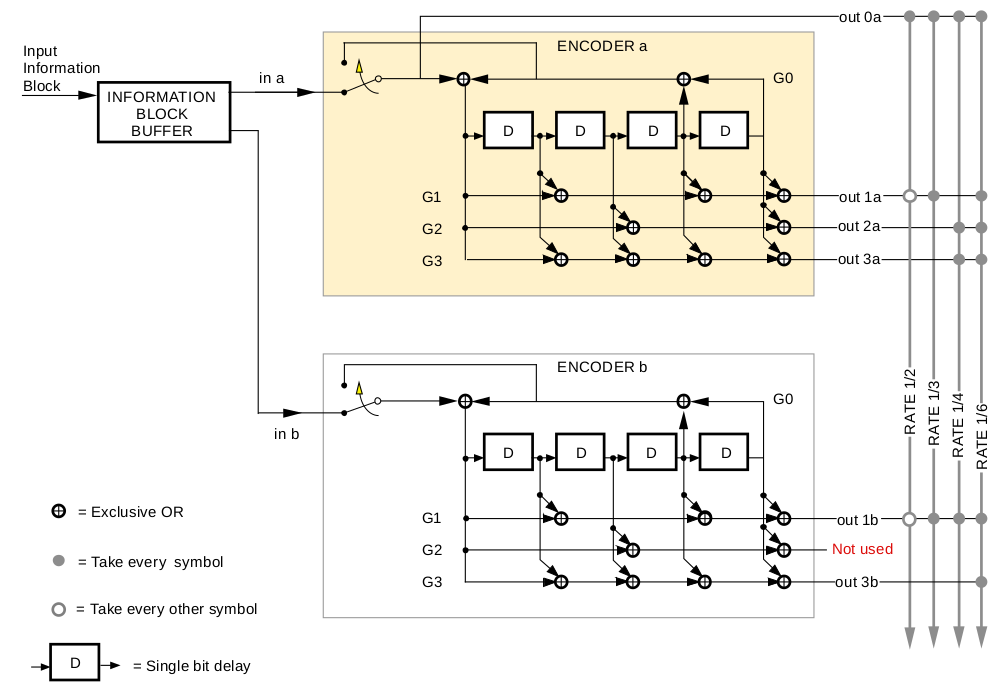
\includegraphics[height=0.75\textheight]{./images/encoder-structure}
    \end{center}
    Convolutional codes defined through forward and backward connection vectors
\end{frame}

%======================================================================================
\begin{frame}[c,fragile]{Example: defining a code in C}
    \begin{lstlisting}[
        language=C,
        basicstyle=\scriptsize,
        commentstyle=\color{mLightGreen},
        stringstyle=\color{mLightRed}
        ]
    // define first code
    int N_components = 2;
    char *forward[N_components];
    forward[0] = "10011";
    forward[1] = "10101";

    char *backward = "0011";

    t_convcode code = convcode_initialize(forward, backward, 
                                            N_components);

    t_turbocode turbo = turbo_initialize(code, code, pi,
                                            info_length);
    \end{lstlisting}
    
\end{frame}
%======================================================================================
\begin{frame}{Interleaver}
    \begin{center}
        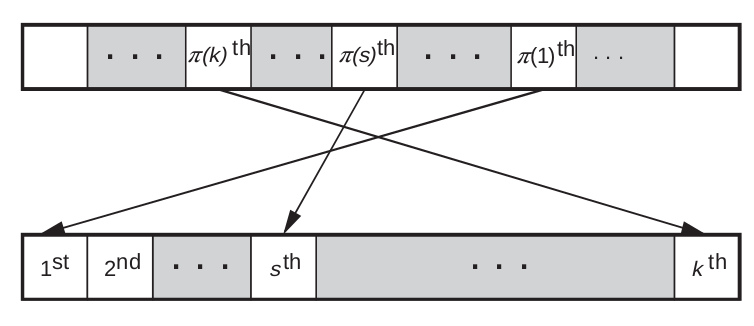
\includegraphics[width=0.5\textwidth]{./images/interleaver}
    \end{center}
    
    $i$-th bit of the interleaved packet is the $\pi(i)$-th bit of the original packet

    \begin{table}
        \centering
        \begin{tabular}{cc}
            \toprule
            Input length $k$ & $k_1 \times k_2 \times k_3$\\
            \midrule
            $1784$    &   $8  \times 223 \times 1$\\
            $3568$    &   $8  \times 223 \times 2$\\
            $7136$    &   $8  \times 223 \times 4$\\
            $8920$    &   $8  \times 223 \times 5$\\
            \bottomrule
        \end{tabular}
    \end{table}
\end{frame}

%======================================================================================
\begin{frame}{Building the interleaver}
    \begin{algorithmic}
        \State $p = \begin{bmatrix}31 & 37 & 43 & 47 & 53 & 59 & 61 & 67\end{bmatrix}$
        \For{$s = 1$ to $k$}
            \State $m = (s-1) \mod 2$
            \State $i = \text{floor}\left[(s-1)/(2k_2)\right]$
            \State $j = \text{floor}\left[(s-1)/2\right] -i k_2$
            \State $t = (19i + 1) \mod (k_1/2)$
            \State $q = t \mod 8 + 1$
            \State $c = (p_q j + 21m) \mod k_2$
            \State $\pi(s) = 2(t + c k_1/2 +1) - m$
        \EndFor
    \end{algorithmic}
\end{frame}

%======================================================================================
\begin{frame}[c]{Decoding}
    \begin{center}
        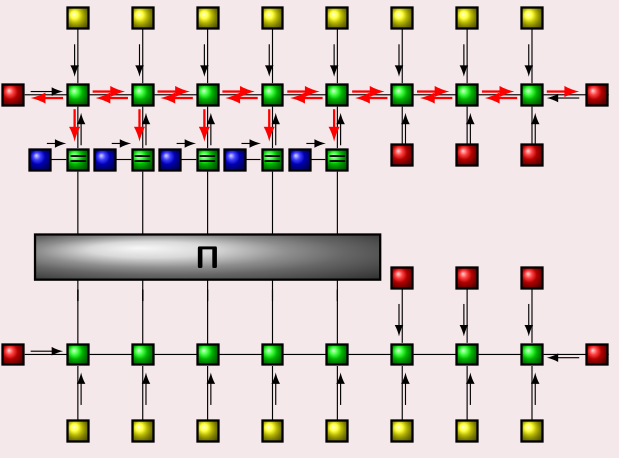
\includegraphics[width=0.5\textwidth]{./images/decoding.png}
    \end{center}
    \begin{itemize}
        \item BCJR (in log domain) on upper and lower code
        \item puncturing is applied at reception 
            $\hat{r}[i] = r[i]\cdot p[i]$ so that
            \[
                g_l(\mathbf{y}_l) \propto \exp\left( -\frac{\Vert \mathcal{L}(\mathbf{y}_l)\Vert^2}{2\sigma_w^2} \right) = \text{const}
            \]
    \end{itemize}
    
\end{frame}
%======================================================================================
\begin{frame}[c,fragile]{Example: defining a code in C}
    \begin{lstlisting}[
        language=C,
        basicstyle=\scriptsize,
        commentstyle=\color{mLightGreen},
        stringstyle=\color{mLightRed}
        ]
        // **messages is initialized to log(0.5)
        int *decoded = NULL;
        for (int i = 0; i < iterations; i++) {

            // run BCJR on upper code
            convcode_extrinsic(streams[0], lengths[0], 
                                 &messages, code.upper_code,
                                 noise_variance, 0);
            // apply interleaver
            message_interleave(&messages, code);

            // run BCJR on lower code
            // save extrinsic messages in **messages
            decoded = convcode_extrinsic(streams[1], lengths[1], 
                                 &messages, code.lower_code, 
                                 noise_variance, 
                                 i == (iterations - 1));
            // deinterleave
            message_deinterleave(&messages, code);
        }
    \end{lstlisting}
\end{frame}
%======================================================================================
% \begin{frame}[c]{Simulator options}
%     \begin{figure}
%         \centering
%        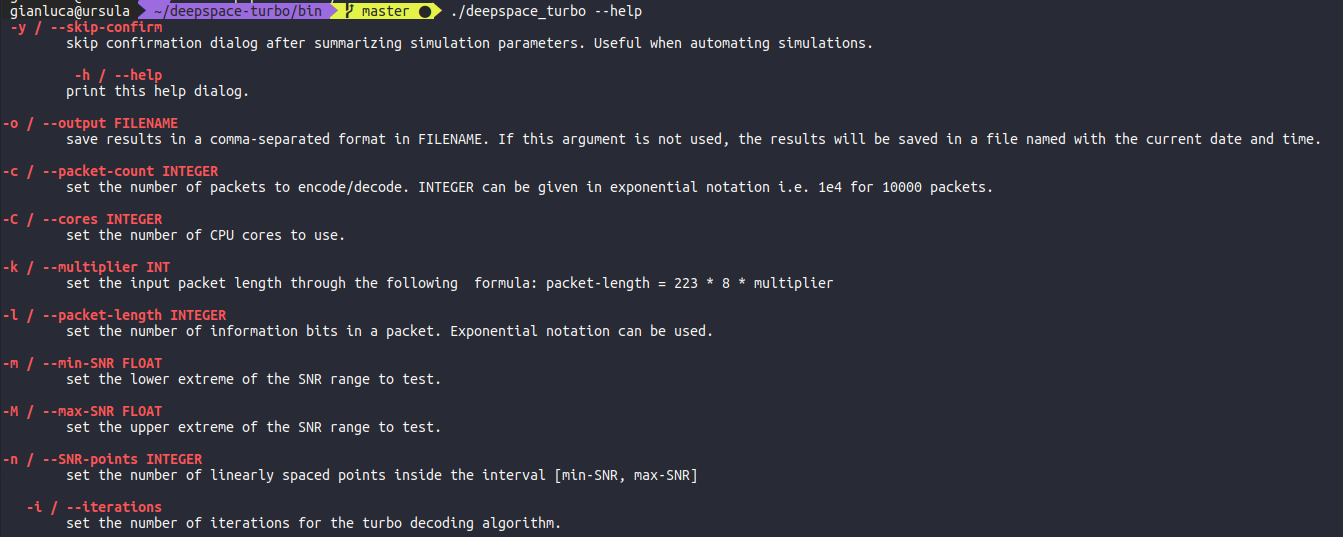
\includegraphics[width=1\textwidth]{./images/terminal}
%     \end{figure}
% \end{frame}
%======================================================================================

%======================================================================================
\begin{frame}[standout]
    \huge Questions?
\end{frame}
% %======================================================================================

\end{document}
